\documentclass[11pt,a4paper]{article}

% ------------------------------------------------------------
% Encoding and page layout
% ------------------------------------------------------------
\usepackage[utf8]{inputenc}
\usepackage[T1]{fontenc}
\usepackage[english]{babel}
\usepackage{geometry}
\geometry{margin=2.5cm}
\usepackage{setspace}
\onehalfspacing

% ------------------------------------------------------------
% Tables, figures, diagrams, links, and code
% ------------------------------------------------------------
\usepackage{graphicx}
\usepackage{booktabs}
\usepackage{longtable}
\usepackage{array}
\usepackage{enumitem}
\usepackage{xcolor}
\usepackage{xurl}
\usepackage{hyperref}
\usepackage{tikz}
\usetikzlibrary{arrows.meta, positioning, shapes.geometric, fit, calc}
\usepackage{listings}

\hypersetup{
    colorlinks=true,
    linkcolor=blue,
    urlcolor=blue,
    citecolor=blue,
    pdftitle={Integration of Ethics and Legality into the Software Pipeline},
    pdfauthor={},
    hypertexnames=false
}

\lstdefinestyle{code}{
    basicstyle=\ttfamily\small,
    breaklines=true,
    frame=single,
    columns=fullflexible,
    keepspaces=true,
    backgroundcolor=\color{gray!5}
}
\lstset{style=code}

\setlist[itemize]{topsep=4pt,itemsep=2pt,parsep=0pt}
\setlist[enumerate]{topsep=4pt,itemsep=2pt,parsep=0pt}

% ------------------------------------------------------------
% TikZ styles
% ------------------------------------------------------------
\tikzset{
    process/.style={rectangle, rounded corners, draw=black, align=center, minimum height=1.0cm, minimum width=2.8cm, fill=gray!8},
    layer/.style={rectangle, rounded corners, draw=black, align=center, minimum height=0.85cm, minimum width=13.5cm, fill=blue!5},
    arrow/.style={-{Latex[length=2.5mm]}, thick},
    smallbox/.style={rectangle, rounded corners, draw=black, align=center, minimum height=0.8cm, minimum width=2.9cm, fill=gray!6},
    gate/.style={diamond, draw=black, align=center, aspect=2.2, fill=orange!12, inner sep=1pt}
}



\begin{document}

% ============================================================
% Dedicated title page
% ============================================================
\begin{titlepage}
    \centering
    \vspace{3.0cm}
    {\huge \textbf{Ethics and Legality Integration into the Agile Software Development Pipeline}\par}
    \vspace{1.5cm}
    {\large Social and Ethical Issues\par}
    \vfill
    {University of Pisa\par}
    {\large \today\par}
\end{titlepage}

% ============================================================
% Dedicated table of contents page
% ============================================================
\pagenumbering{roman}
\thispagestyle{plain}
\tableofcontents
\clearpage

% ============================================================
% Main text
% ============================================================
\pagenumbering{arabic}


\section{Introduction}

Modern software systems increasingly operate as socio-technical infrastructures: they do not merely execute functions, but mediate access to services, process personal data, automate decisions, and shape organisational behaviour. For this reason, a software pipeline cannot be evaluated only in terms of functional correctness, delivery speed, or security. It must also make ethical values and legal obligations explicit, traceable, testable, and monitorable.

This report proposes a progressive engineering model for integrating ethics and legality into a contemporary software development DevOps pipeline. The model starts from an Agile sprint loop in which the most of the backward arrows are implicit because of the iterative nature of Agile development and to simplify the diagram.

The Agile loop is expanded through four layers:

\begin{enumerate}
    \item \textbf{Agile based on Value Sensitive Design (VSD) and Conceptual Engineering (CE)} \cite[Ch.~13]{umbrello_agile_vsd}, \cite[Secs.~2--4]{veluwenkamp_ce}: values and stakeholders enter the backlog, while ambiguous values are clarified before becoming requirements.
    \item \textbf{GORE + SLEEC} \cite[Secs.~3--4]{silva_gore_sleec}: values become normative goals and then formal, testable rules.
    \item \textbf{Compliance-as-Code (CaC)} \cite[Sec.~Implementation]{bml_ethsecdevops}, \cite[Secs.~3--4]{potharalanka_cac}, \cite[Secs.~4--5]{singh_cac}: ethical and legal requirements are enforced through CI/CD gates, policy engines, and audit evidence.
    \item \textbf{MLOps + Runtime Assurance} \cite[Secs.~3--5]{lu_responsible_ai}, \cite[Secs.~5.2.3--5.2.5 and~9.2.3]{taid_whitepaper}: AI-specific risks are controlled through model evaluation, monitoring, and human oversight.
\end{enumerate}

The central thesis is that responsible software engineering requires a shift from \emph{late ethical review} to \emph{continuous ethical and legal assurance}.


\section{Conceptual Foundations}

\subsection{Cybernetics: feedback as the organising principle}

The proposed pipeline is cybernetic in structure \cite[Ch.~4]{wiener_cybernetics}. It is organised around feedback loops that compare observed behaviour with desired goals and then correct the system or the process. Agile retrospectives, CI test failures, policy violations, model drift alerts, incident postmortems, and human override mechanisms all instantiate negative feedback.

This matters because ethical and legal compliance cannot be treated as a static checklist. Values evolve, stakeholders reinterpret impacts, operational environments change, and AI models degrade or behave unexpectedly. Therefore, the pipeline must repeatedly evaluate also if the system still satisfies its goals.

\subsection{The limits of the intelligence imitation of modern machines}

The Turing-test tradition frames intelligence behaviourally \cite[Sec.~1]{turing_computing}: a machine may appear intelligent if its outputs are indistinguishable from those of a human. However, software engineering for responsible AI cannot rely only on output imitation. A system may produce convincing behaviour while still violating privacy, amplifying bias, or hiding causal responsibility. The distinction between weak and strong AI is therefore operationally relevant: most deployed AI systems should be engineered as powerful decision-support artefacts, not as autonomous moral subjects.

Also the Searle's Chinese Room argument is useful as a warning for formal compliance \cite[pp.~417--420]{searle_chinese_room}. A rule engine may manipulate symbols correctly while lacking semantic understanding of the underlying value. This is not an argument against formalisation; rather, it shows why formal rules must remain connected to stakeholder interpretation, domain expertise, legal review, and human oversight. In the proposed pipeline, SLEEC rules and policy-as-code are therefore treated as \emph{engineering artefacts requiring governance}, not as replacements for judgement.

\subsection{Responsibility and the Problem of Many Hands}

\textbf{Active responsibility} becomes operational through blocking controls: the pipeline prevents non-compliant artefacts from reaching production. \textbf{Passive responsibility} becomes operational through evidence: every policy decision, exception, deployment, and runtime alert is logged for later audit and accountability. Both are needed because development requires forward-looking prevention, while deployment requires reconstructable evidence when a release, model, monitor, or human override must be reviewed after the fact.

This directly addresses the many-hands problem. Instead of relying on memory or informal coordination, the pipeline records decisions and makes responsibility attributable at the artefact level.

Modern pipelines distribute action across product owners, developers, data engineers, security engineers, ML engineers, legal teams, platform teams, policy engines, and runtime systems. This generates the classic problem of ``many hands'': outcomes are collectively produced, but accountability can become diffuse. In AI systems, this may create a \textbf{responsibility gap}, especially when decisions emerge from blackbox models from which is hard to identify a responsible party \cite[pp.~175--182]{matthias_responsibility_gap}.

The pipeline proposed in this report addresses the responsibility gap by introducing
an explicit \textbf{RACI Matrix} after the definition of the \textit{Sprint Backlog} and before
the CI/CD pipeline. Once the value-derived norms, GORE/SLEEC rules, technical tasks,
and compliance controls have been selected for the sprint, the RACI Matrix assigns
clear responsibility roles to the relevant actors.
Responsible is the actor who performs the task or implements the control;
Accountable is the actor who owns the final decision or approval;
Consulted are the actors whose expertise is required, such as legal, ethics, domain, or security experts;
Informed are the actors who must be kept aware of decisions, failures, exceptions, or residual risks.

In this way, responsibility is not left implicit in the technical pipeline.
This reduces the risk that accountability becomes diffuse across the many actors
involved in the development and operation of an AI-enabled software system.
It also connects active responsibility to the actors who must prevent failures during development, and passive responsibility to the actors who must justify decisions after deployment.


\section{Value Sensitive Design in Agile}

\subsection{The Agile loop}

The initial diagram is a standard Agile loop, of which an example can be found in Figure~\ref{fig:agile-loop}. Its strength is rapid iteration, while its weakness is that values may remain implicit unless they are deliberately introduced into sprint artefacts. For simplicity, the figure shows the main delivery flow; the backward feedback from review and retrospective into \textit{Backlog Refinement} and \textit{Sprint Planning} is implicit in the Agile loop. For this reason, the backlog is not treated only as a queue of features: it is the first place where affected stakeholders, data sources, legal constraints, and foreseeable harms must become visible engineering inputs.

\begin{figure}[ht]
\centering
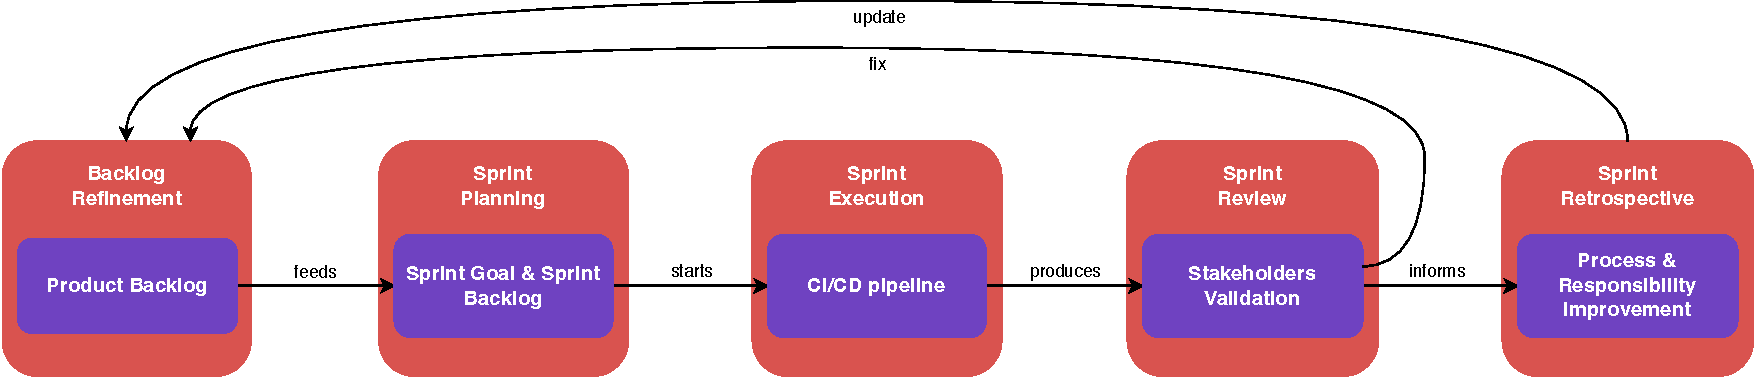
\includegraphics[width=0.70\textwidth]{../diagram/agile1.pdf}
\caption{Baseline Agile/Scrum sprint loop, used as the starting point for the progressive integration of ethical and legal assurance.}
\label{fig:agile-loop}
\end{figure}

\subsection{Stakeholder tokens and value source analysis}

Within the proposed pipeline, stakeholder tokens and value source analysis are both performed inside the \textit{Value Elicitation} activity of the \textit{Backlog Refinement} phase. This activity is not intended to produce final technical requirements directly. Rather, it enriches the backlog with an explicit understanding of the actors affected by the system and of the values that should constrain the resulting user stories.

Stakeholder tokens make affected actors visible during discussion, preventing the team from considering only the primary user or the customer. In this report, they are interpreted as a practical way to keep track of direct users, data subjects, maintainers, regulators, vulnerable groups, non-users, and indirectly affected communities while backlog items are being refined.

Value source analysis complements this by clarifying where the relevant values originate. These sources may include stakeholder expectations, legal requirements, organisational principles, professional codes, domain standards, social expectations, and risk assessments. In practice, stakeholder tokens help identify whose interests must be represented, while value source analysis explains why values such as privacy, fairness, transparency, or autonomy should constrain specific user stories.

The output of \textit{Value Elicitation} is therefore a set of values associated with the backlog which are transformed into norms (as we'll see in the next chapters) and then into user stories. Then they can be clarified through Conceptual Engineering and refined into GORE/SLEEC requirements.

\subsection{Conceptual Engineering}

A value such as privacy, autonomy, transparency, or fairness is too abstract to be directly implemented; so, different conceptualisations of the same value can imply different technical requirements. The Design for Values and Conceptual Engineering literature argues that value-based requirements engineering needs systematic conceptual work because different conceptions of abstract values lead to different design requirements \cite[Secs.~2--4]{veluwenkamp_ce}. This is also where the pipeline protects itself against purely syntactic compliance: a term may be accepted by a rule or a ticket template while still being semantically unclear for stakeholders, regulators, or operators.

During sprint planning, the team should run a short conceptual clarification step:

\begin{enumerate}
    \item \textbf{Discovery}: how is the value currently understood by stakeholders and in the domain?
    \item \textbf{Justification}: does the current concept serve the intended moral, legal, and engineering function?
    \item \textbf{Construction}: which refined conception should be adopted for this system?
\end{enumerate}

In the integrated diagrams, this is represented by the \textit{Discovery phase}, \textit{Justification phase}, and \textit{Construction phase} inside \textit{Sprint Planning}. The loop is deliberately placed before the \textit{Sprint Backlog} is fixed: discovery gathers how a value is currently used, justification checks whether that use serves the moral, legal, and engineering purpose, and construction records the clarified concept that the team will implement. This prevents ambiguous values from silently becoming ambiguous requirements.

\subsection{First value hierarchy}

The first stable artefact is a value hierarchy. It is produced during \textit{Sprint Planning}, after \textit{Value Elicitation} has identified relevant values and Conceptual Engineering has clarified their meaning. Therefore, it is not yet a GORE model or a SLEEC rule: it is the bridge that connects each abstract value to a more concrete norm, then to a design requirement, and finally to a verification artefact that can be checked during development. Appendix Table~\ref{tab:value-hierarchy-examples} gives illustrative examples.

For GDPR-relevant systems, this hierarchy has legal implications because the chosen norms must preserve Article~5 principles such as lawfulness, fairness, transparency, purpose limitation, data minimisation, accuracy, storage limitation, integrity/confidentiality, and accountability, and must support Article~25 data protection by design and by default \cite[Art.~5]{gdpr_art5}, \cite[Art.~25]{gdpr_art25}, \cite[Secs.~2--3]{edpb_dpbdd}. For AI systems, the same hierarchy also prepares later controls for the AI Act's risk-based framework and for human oversight of high-risk AI systems \cite[Sec.~Risk-based approach]{eu_ai_act}, \cite[Art.~14]{ai_act_human_oversight}. In practice, this means that a value such as privacy or autonomy must already be traceable before it becomes a \textit{GORE Normative Goals} item, a \textit{SLEEC Rules} item, or a policy gate.

\subsection{Integration with the Agile model}

Value Sensitive Design and Conceptual Engineering are useful here because are not an external ethical audit added after implementation. It is a design approach that incorporates human values throughout design work. The Agile-VSD literature argues that VSD can be integrated into existing Agile workflows rather than replacing them; values can be represented and refined inside sprint planning, model evaluation and backlog management \cite[Secs.~13.4--13.5]{umbrello_agile_vsd}. Figure~\ref{fig:agile-vsd} shows this integration by connecting stakeholder analysis, \textit{Value Elicitation}, value-sensitive implementation, testing, review, and retrospective updates to the normal sprint loop. The added \textit{AI Risks \& Data Sources} input makes the pipeline sensitive to a central problem of data-driven systems: behaviour may look correct while the underlying data selection, measurement categories, or optimisation target still encode bias, opacity, or privacy risk.

\begin{figure}[ht]
\centering
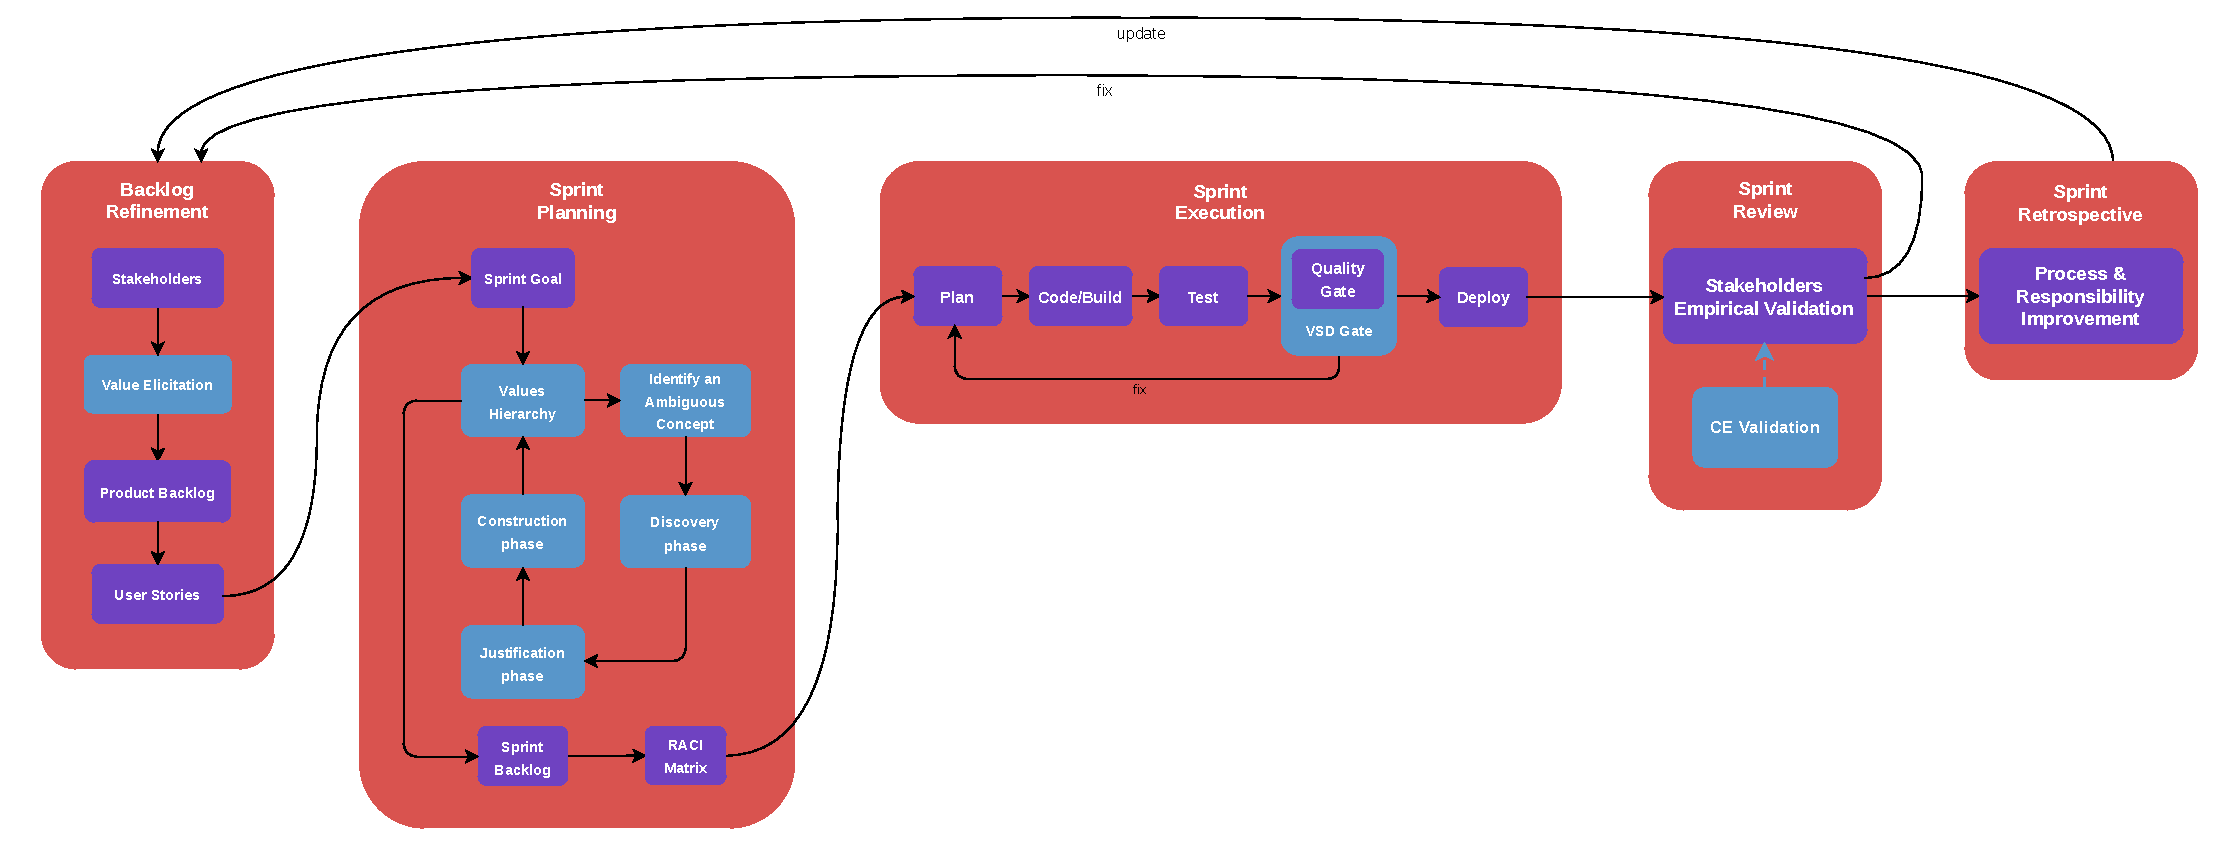
\includegraphics[width=0.80\textwidth]{../diagram/agile3.pdf}
\caption{Agile/Scrum sprint loop enriched by Value Sensitive Design, showing how ethical reflection becomes part of ordinary iterative development.}
\label{fig:agile-vsd}
\end{figure}


\section{Requirements Engineering through GORE and SLEEC}

\subsection{From values to Norms}

The next expansion of the model moves from value analysis to requirements engineering. Goal-Oriented Requirements Engineering (GORE) is used to represent stakeholder intentions as goals. In the ethics-aware adaptation literature, ethical values are represented as \textbf{normative goals} aligned with functional and adaptation goals, enabling analysis of trade-offs and conflicts \cite[Sec.~3]{silva_gore_sleec}. In this stage, values are transformed into normative goals, connected to functional or adaptation goals, decomposed into tasks, and finally expressed as rules that can be reviewed and tested. GORE gives the pipeline a place to ask why a requirement exists, not only what the system must do; this matters when competing goals such as privacy, safety, usability, and accountability cannot all be maximised at the same time.

\subsection{GORE artefacts}

A GORE model should distinguish the following types of goals and conditions \cite[Sec.~3]{silva_gore_sleec}:

\begin{itemize}
    \item \textbf{Normative goals}: obligations grounded in values, law, or institutional principles.
    \item \textbf{Functional goals}: services the system must provide.
    \item \textbf{Adaptation goals}: how the system changes behaviour under context changes.
    \item \textbf{Obstacles}: conditions that prevent goal satisfaction.
    \item \textbf{Trade-offs}: when there are conflicts between goals (e.g. privacy versus safety).
\end{itemize}

\subsection{From normative goals to SLEEC rules}

SLEEC rules translate normative goals into a form that is close to natural language but structured enough for automated analysis. In the cited SLEEC work, rules have the general form ''\texttt{when <condition> then <response> [within <time>] [unless <exception>]}'' \cite[Sec.~4]{silva_gore_sleec}. In the pipeline, \textit{SLEEC Rules} are the bridge between ethical language and executable control: they keep rules understandable for human review while making triggers, responses, deadlines, and exceptions precise enough for tests and monitors. Appendix Listings~\ref{lst:sleec-erasure} and~\ref{lst:sleec-human-review} give two illustrative examples.

\subsection{Testability and conflict detection}

SLEEC-style rules improve engineering quality because they support well-formedness checking, conflict detection between rules, mapping to acceptance tests, mapping to runtime monitors, and review by non-technical stakeholders. In fact it can be viewed as a bridge between the ethical language of values and the technical language of code, allowing a better communication between developers and stakeholders.

This stage is where values become technically actionable. However, the Chinese Room argument still applies: formal rules must remain explainable and reviewable, because syntactic rule execution does not guarantee semantic adequacy.

\subsection{Integration with the Agile-VSD model}

Figure~\ref{fig:gore-sleec-detail} shows how the Agile-VSD loop is extended with a requirement engineering branch. Conceptual Engineering clarifies values during \textit{Sprint Planning}, \textit{GORE Normative Goals} turn them into normative goals, and \textit{SLEEC Rules} make them precise enough to feed the \textit{Sprint Backlog}. The diagram therefore makes responsibility assignable: each value is transformed into a concept (CE), each concept into one or more normative goals (GORE), and for each one a rule is written (SLEEC).

\begin{figure}[ht]
\centering
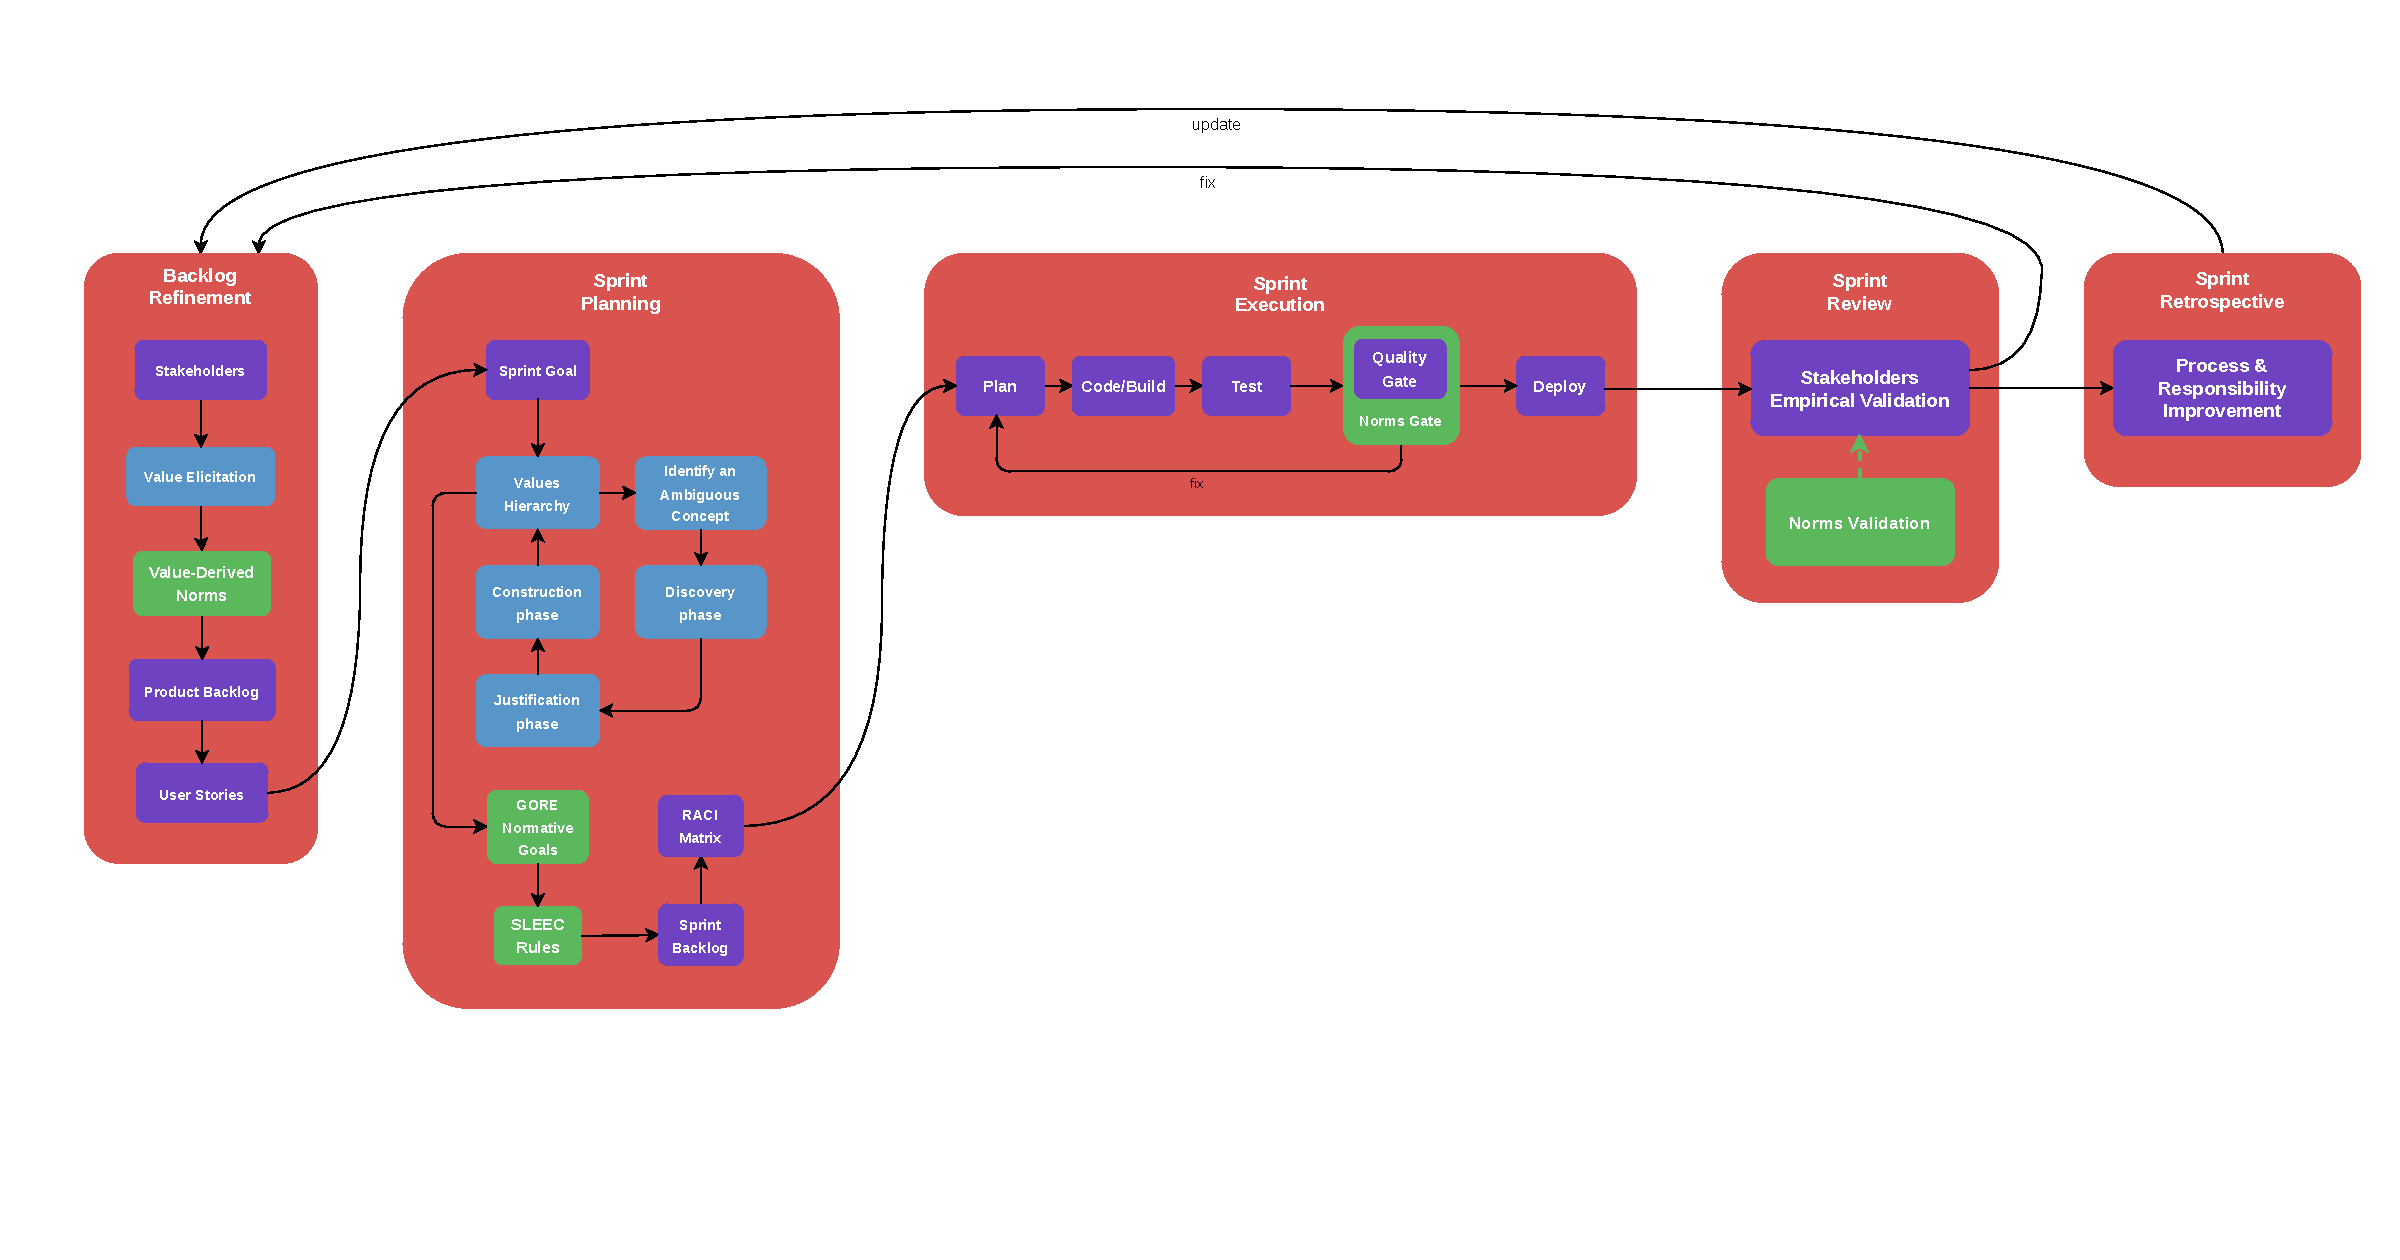
\includegraphics[width=0.80\textwidth]{../diagram/agile5.pdf}
\caption{Detailed planning view showing how clarified values are transformed into operational requirements before implementation starts.}
\label{fig:gore-sleec-detail}
\end{figure}


\section{DevOps and Compliance-as-Code}

\subsection{From ethical requirements to pipeline controls}

The next expansion shifts the focus from requirements specification to the DevOps CI/CD pipeline. Compliance-as-Code (CaC) expresses legal and organisational compliance requirements as executable, version-controlled, testable policy artefacts. The CaC literature describes this as a shift from document-centric and retrospective compliance toward programmatic controls embedded directly in the software delivery lifecycle \cite[Secs.~2--4]{potharalanka_cac}, \cite[Secs.~3--5]{singh_cac}.

\subsection{Shift-left compliance}

Shift-left compliance means that checks are executed as early as possible, ideally before code reaches production. CaC should be integrated at multiple points, as defined in Appendix Table~\ref{tab:cac-controls}.

The Deployflow source describes an audit-ready DevOps pipeline as a pipeline that does not rely on manual evidence collection after the fact. Instead, it automatically records relevant actions, preserves tamper-resistant evidence, controls access through Role-Based Access Control (RBAC), enforces security measures such as encryption, monitors the system continuously, and produces audit reports from the information already collected during development and deployment. In this sense, the pipeline makes each change repeatable, traceable, and auditable \cite[Sec.~Audit-Ready Pipelines in Action]{deployflow_gdpr}. The EthSecDevOps article published by BML Global reinforces the same direction from an ethical perspective: ethics should be treated as a first-class concern, with early value assessment, stakeholder analysis, ethical code reviews, fairness testing, ethical deployment checklists, and continuous monitoring \cite[Secs.~Implementing Ethics in the Development Pipeline and Deployment and Operations]{bml_ethsecdevops}.

\subsection{Policy-as-Code tools}

Policy-as-Code tools such as Open Policy Agent (OPA), HashiCorp Sentinel, Chef InSpec, and Cloud Custodian can express compliance constraints in executable form. In the model, these tools populate the \textit{CaC Policy Library} rather than acting as isolated scripts. A retention rule, an encryption rule, or an access-control rule becomes part of a governed repository that can be tested, reviewed, versioned, and connected to audit evidence. Appendix Listings~\ref{lst:opa-encryption} and~\ref{lst:opa-retention} show two illustrative examples.

\subsection{Integration with the Agile Normative-based model}

The previous requirements branch is connected to CI/CD gates. \textit{GORE Normative Goals} and \textit{SLEEC Rules} become policy-as-code checks, those checks block or approve pipeline stages, and their decisions are stored as audit evidence. The \textit{CaC Policy Library} in the diagram is the versioned memory of these rules: it prevents compliance from depending on informal recollection and makes policy changes reviewable like source code. The \textit{Compliance Gate} is the point where the pipeline acts, because a failed legal, security, or ethical control can stop a release before harm reaches production. The \textit{Audit Evidence Store} gives the same process a backward-looking function, preserving policy decisions, exceptions, and deployment records.

\begin{figure}[ht]
\centering
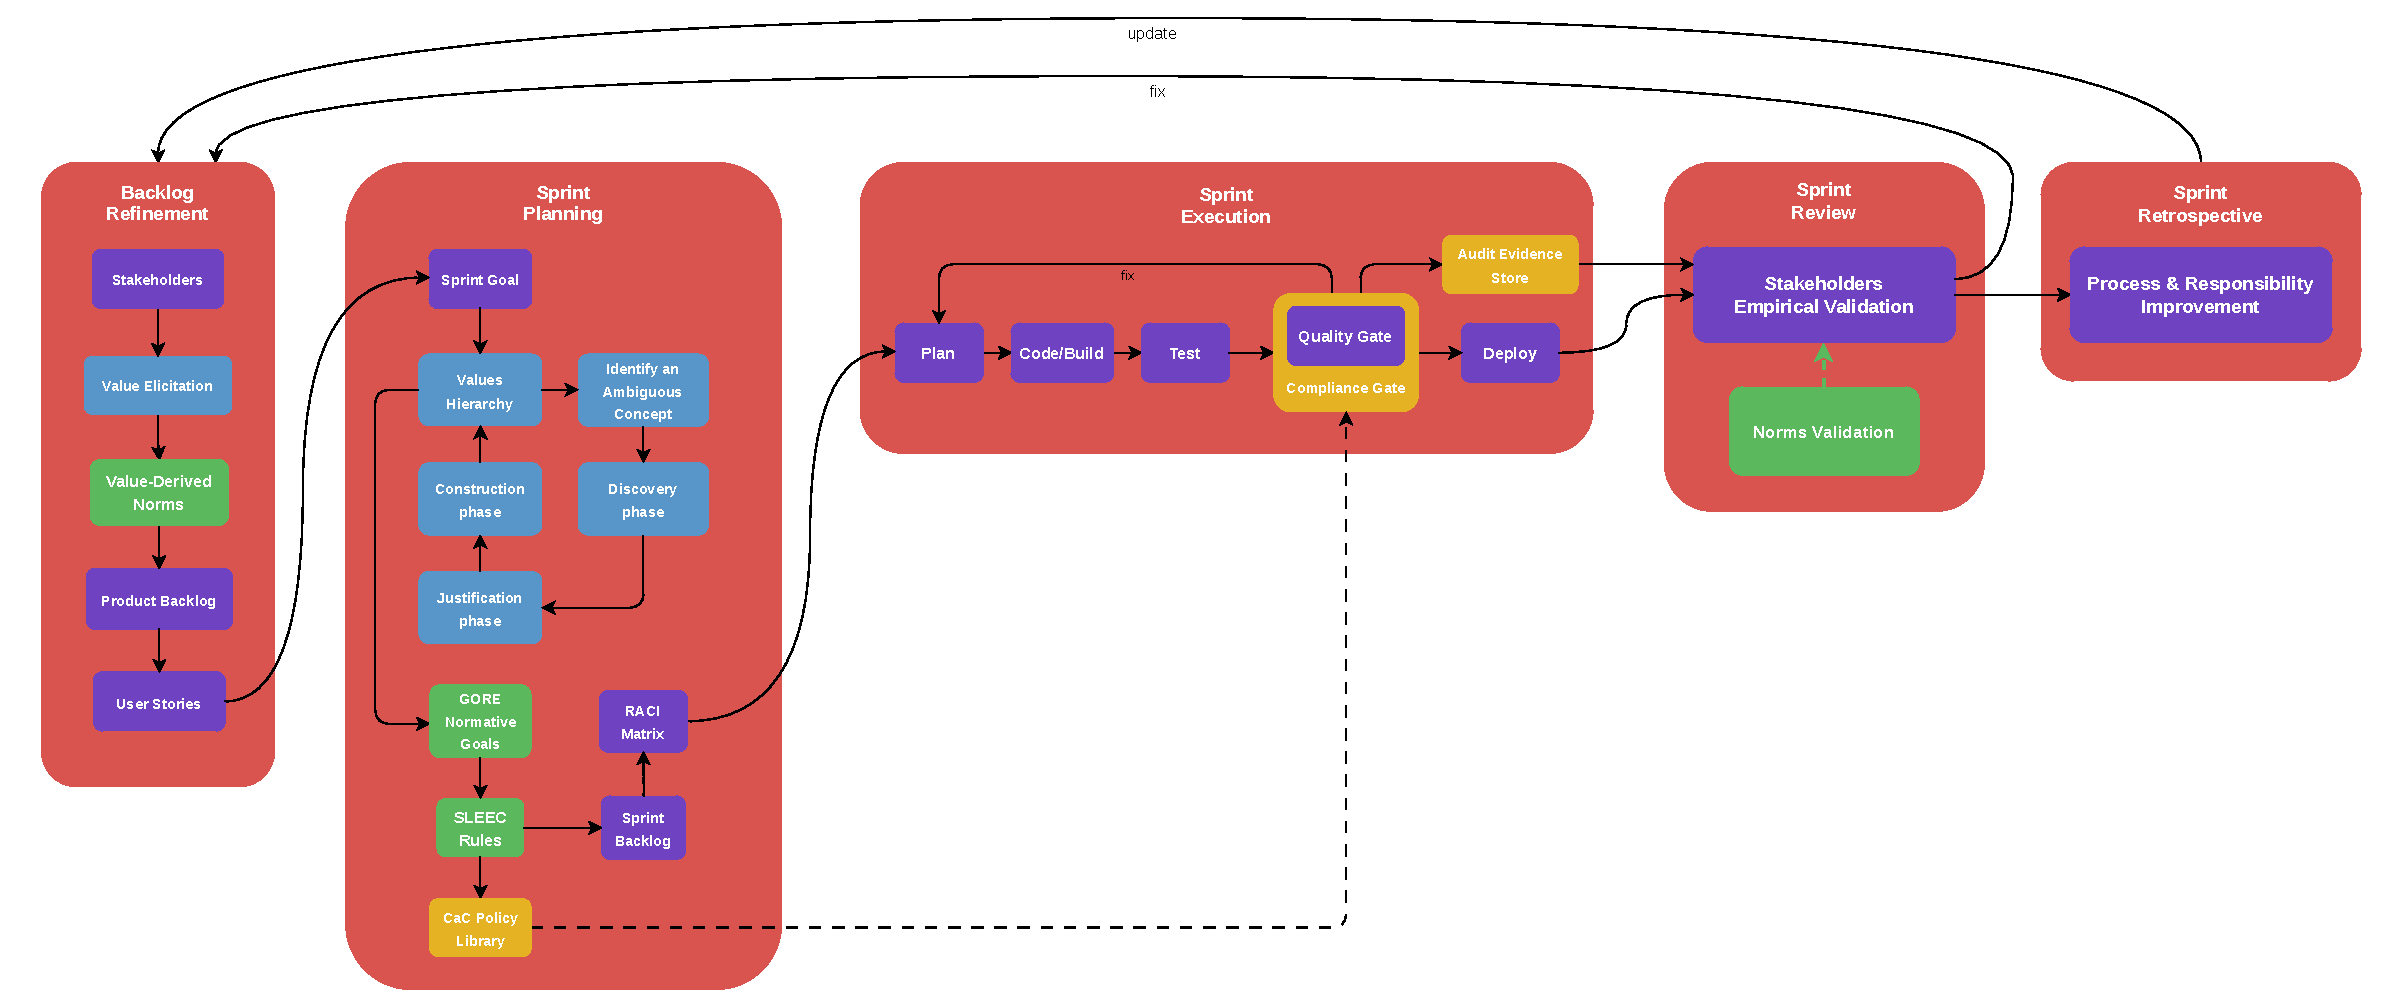
\includegraphics[width=0.80\textwidth]{../diagram/agile7.pdf}
\caption{CI/CD expansion showing how compliance checks and audit evidence become part of the delivery process.}
\label{fig:cac-pipeline}
\end{figure}


\section{MLOps and Runtime Assurance}

\subsection{Why AI requires a further expansion}

AI systems add new sources of risk: training data may be biased, model behaviour may be statistically uncertain, the operational environment may diverge from the training environment, and performance may degrade after deployment. The responsible-AI software engineering roadmap highlights that responsible AI must be operationalised across governance, process, and system perspectives, not only at the algorithm level \cite[Secs.~3--5]{lu_responsible_ai}. It also emphasises continuous and iterative monitoring, co-versioning of data/model/code/configuration, audit trails, and dynamic ethical risk assessment during operation \cite[Sec.~4.1]{lu_responsible_ai}. The \textit{AI Risks \& Data Sources} block in the diagram expresses this shift: responsible AI begins before model training, when the team decides which data sources are legitimate, which affected groups may be represented or excluded, and which risks must enter the backlog.

For AI systems, the DevOps pipeline must also manage data, training, validation, deployment, runtime monitoring, and possible retraining or rollback.

\subsection{The W-shaped AI lifecycle}

For AI systems, especially high-risk systems, the W-shaped lifecycle is more appropriate than a simple V-model. The TAID white paper describes the AI W-shape as an expansion of the traditional V-model that accounts for the specificities of AI constituents, including the tight connection between the AI model and its pre/post-processing \cite[Sec.~5.2.3]{taid_whitepaper}. It distinguishes the \textit{host platform}, where the AI model and software system are developed, trained, tested, and validated before deployment, from the \textit{target platform}, where the deployed AI-enabled system operates under real runtime conditions and requires monitoring, human oversight, and assurance mechanisms \cite[Secs.~5.2.4--5.2.5]{taid_whitepaper}.

\subsection{Design-time assurance}

As shown in Appendix Figure~\ref{fig:mlops-assurance}, design-time assurance takes place before deployment. Its purpose is to check whether the AI component is sufficiently reliable, compliant, and fit for the operational context in which it will be used. It includes checks on data quality and lineage, bias and representativeness, model validation, robustness and generalisation, explainability, and conformity with legal or organisational policies.

The key additional control is the \textit{Model Evaluation Gate}. This gate ensures that a trained model is not accepted simply because it can be executed, but only if there is enough evidence that it satisfies its requirements and that the remaining risks are understood.

In this sense, design-time assurance mainly supports active responsibility: foreseeable harms must be identified, assessed, and mitigated before the model is deployed.

\subsection{Runtime assurance}

Runtime assurance is performed after deployment and focuses on whether the deployed system remains trustworthy under actual operating conditions. Appendix Figure~\ref{fig:mlops-assurance} separates the \textit{Runtime Assurance} layer from the design-time gates and shows the monitoring and control mechanisms that remain active after deployment. Data drift monitoring checks whether input distributions have changed, concept drift monitoring checks whether the relation between inputs and outputs has shifted, and performance monitoring follows accuracy, latency, error rates, and fairness metrics. Safety-envelope monitoring detects states outside the approved operational domain, while fallback mechanisms, rollback, conservative decision logic, and human escalation turn monitoring into corrective feedback rather than passive observation.

Runtime assurance supports both active and passive responsibility. It actively prevents uncontrolled degradation and passively produces evidence for incident reconstruction.

\subsection{Meaningful Human Control}

\textit{Meaningful Human Control} (MHC) is the mechanism that prevents technological autonomy from eliminating human accountability. The TAID white paper identifies MHC as a key open issue for trustworthy AI and links it to compliance, dignity, and responsibility \cite[Secs.~6.3 and~7.1.4]{taid_mhc}. In the pipeline, MHC is integrated after \textit{Runtime Assurance}: monitors detect uncertainty, drift, safety-envelope violations, or high-impact decisions, and explicit escalation thresholds route those cases to a human operator. This avoids treating human oversight as a symbolic approval step. The main risks are that operators may lack enough context, may over-trust the model recommendation, may have no real authority to stop the system, or may be asked to approve too many decisions too quickly. For this reason, MHC must be engineered through interfaces that provide context and explanation, authority to override or stop the system, logging of human decisions and machine recommendations, and clear training and role definitions for operators.

\subsection{Final Agile Normative \& Risk-prevention based model}

In Figure~\ref{fig:final-pipeline}, the \textit{AI Risks \& Data Sources} inputs enter \textit{Backlog Refinement} before \textit{Sprint Planning}, so the system starts from the people, data, and harms that may be affected. \textit{Sprint Planning} then contains the CE loop, where ambiguous values are clarified before they become engineering commitments. \textit{GORE Normative Goals} and \textit{SLEEC Rules} translate those commitments into goals and rules, the \textit{CaC Policy Library} stores the executable policy version of those rules, and the \textit{Compliance Gate} checks them during delivery. The \textit{Audit Evidence Store} preserves the decisions produced by these gates, while the \textit{Model Evaluation Gate} and \textit{Runtime Assurance} blocks keep the AI component under control before and after deployment.

\begin{figure}[ht]
\centering
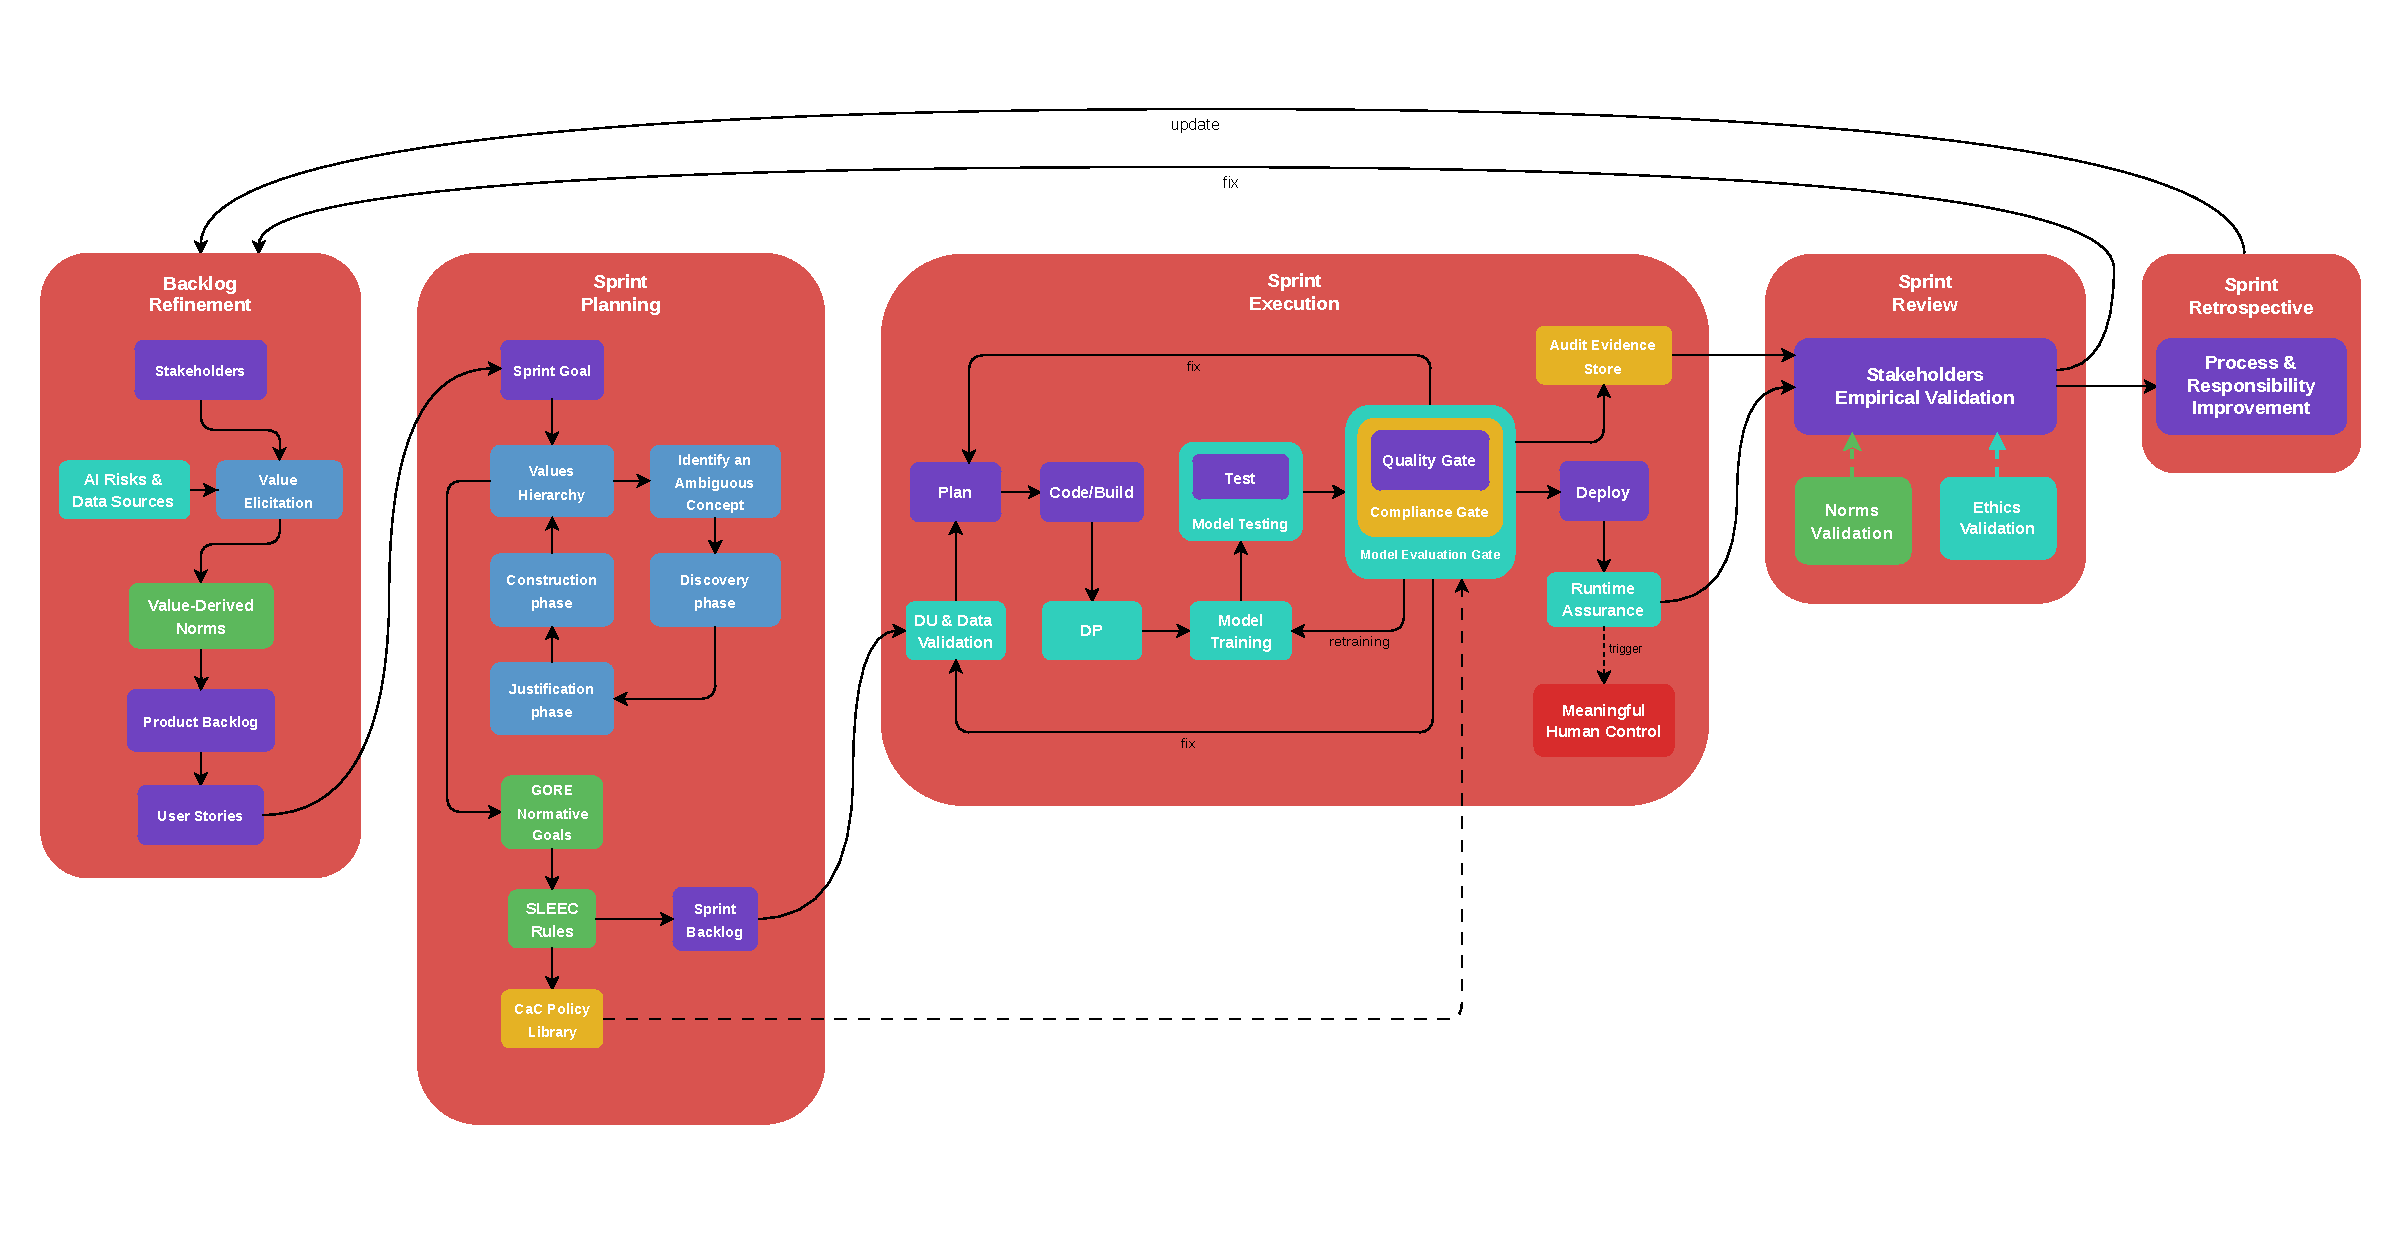
\includegraphics[width=0.80\textwidth]{../diagram/agile9.pdf}
\caption{Final pipeline with the full progression from value elicitation to design-time and runtime assurance related to the MLOps integration.}
\label{fig:final-pipeline}
\end{figure}


\section{Conclusions}

The final pipeline transforms ethics and legality from abstract external concerns into engineering artefacts. Agile provides the iterative structure; VSD introduces stakeholders and values; Conceptual Engineering clarifies the meaning of those values; GORE and SLEEC operationalise them as goals and rules; Compliance-as-Code enforces them in the CI/CD pipeline; MLOps and Runtime Assurance keep AI systems aligned after deployment.

The result is a pipeline oriented toward \textbf{socio-technical trustworthiness}. It does not guarantee perfect ethical behaviour, but it creates a disciplined framework for making values explicit, legal obligations traceable, compliance testable, runtime behaviour observable, and responsibility attributable.


\clearpage
\appendix

\section{MLOps Assurance Diagram}

\begin{figure}[ht]
\centering
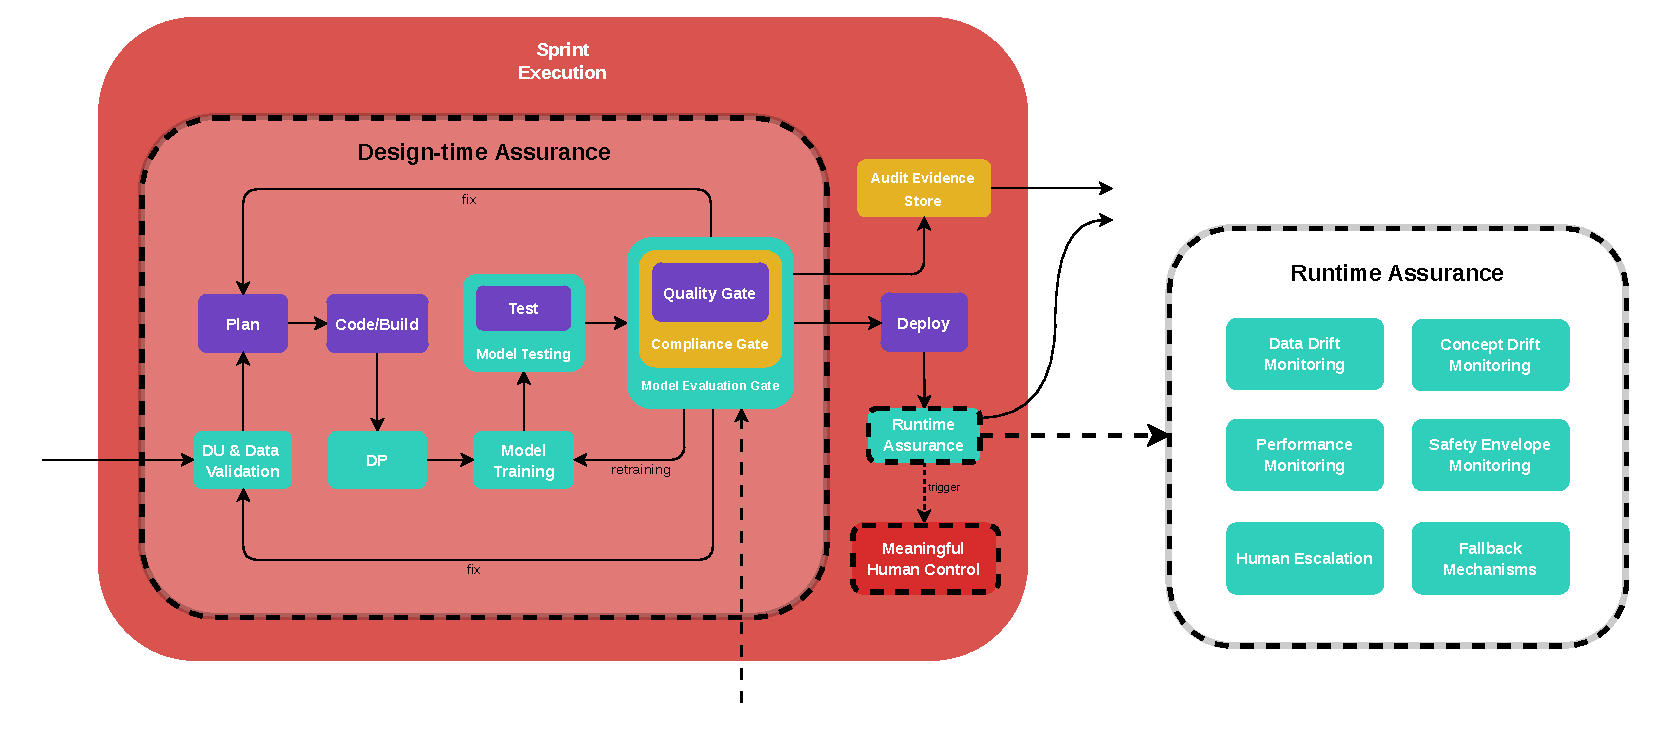
\includegraphics[width=\textwidth]{../diagram/agile10.pdf}
\caption{MLOps assurance view, distinguishing the checks performed before deployment from the monitoring and control mechanisms active after release.}
\label{fig:mlops-assurance}
\end{figure}

\section{Value Hierarchy Examples}

\begin{table}[ht]
\centering
\begin{tabular}{p{2.4cm}p{3.4cm}p{5.0cm}p{3.5cm}}
\toprule
\textbf{Value} & \textbf{Norm} & \textbf{Requirement} & \textbf{Verification} \\
\midrule
Privacy & Data minimisation & Collect only fields required for the declared purpose. & Schema test; privacy review \\
Autonomy & Meaningful user control & Provide users with the ability to change their choices or appeal decisions. & UX test; audit log \\
Fairness & Non-discrimination & Evaluate model performance across relevant groups. & Fairness test report \\
Transparency & Explainability & Provide understandable reasons for consequential decisions. & Explanation acceptance test \\
Security & Integrity and confidentiality & Encrypt personal data at rest and in transit. & IaC/policy test \\
\bottomrule
\end{tabular}
\caption{Illustrative examples of value hierarchy entries.}
\label{tab:value-hierarchy-examples}
\end{table}

\section{SLEEC Rule Examples}

\begin{lstlisting}[caption={Example SLEEC-style rule for GDPR deletion.},label={lst:sleec-erasure}]
rule delete_personal_data:
  when UserRequestsErasure and requestIsValid
  then DeletePersonalData within 30 days
  unless legalRetentionObligation
  then RestrictProcessing and NotifyUser within 7 days
\end{lstlisting}

\begin{lstlisting}[caption={Example SLEEC-style rule for human oversight.},label={lst:sleec-human-review}]
rule human_review_high_risk_decision:
  when HighRiskAIDecisionGenerated and confidence < threshold
  then EscalateToHumanReviewer within 5 minutes
\end{lstlisting}

\section{Compliance-as-Code Examples}

\begin{longtable}{p{3.0cm}p{5.0cm}p{5.0cm}}
\caption{Compliance controls across the CI/CD pipeline.}\label{tab:cac-controls}\\
\toprule
\textbf{Pipeline stage} & \textbf{Typical controls} & \textbf{Evidence produced} \\
\midrule
Code / pre-commit & secret detection, linting, privacy annotations, prohibited API checks & commit metadata, static-analysis report \\
Build & dependency scanning, licence checks, reproducible build & SBOM, dependency report, build signature \\
Test & privacy tests, fairness tests, security tests, SLEEC-derived acceptance tests & test report, model-card update, risk record \\
Release gate & OPA/Sentinel policy evaluation, approval workflow, exception handling & policy decision log, approver identity \\
Deploy & infrastructure-as-code validation, RBAC, encryption, network controls & deployment manifest, IaC compliance report \\
Operate & runtime monitoring, audit logs, drift detection, incident alerts & immutable logs, alert history, incident timeline \\
\bottomrule
\end{longtable}

\begin{lstlisting}[caption={Illustrative OPA/Rego-style encryption rule.},label={lst:opa-encryption}]
deny[msg] {
  input.resource.type == "database"
  not input.resource.encryption_at_rest
  msg := "Database must enable encryption at rest."
}
\end{lstlisting}

\begin{lstlisting}[caption={Illustrative OPA/Rego-style retention rule.},label={lst:opa-retention}]
deny[msg] {
  input.dataset.contains_personal_data
  input.dataset.retention_days > input.policy.max_retention_days
  msg := "Personal-data retention exceeds the approved policy."
}
\end{lstlisting}

\section{Traceability matrix}

\begin{longtable}{p{2.5cm}p{3.1cm}p{3.4cm}p{3.8cm}}
\caption{End-to-end traceability from value to operational evidence.}\\
\toprule
\textbf{Level} & \textbf{Artefact} & \textbf{Example} & \textbf{Evidence} \\
\midrule
Value & Value statement & Privacy must be preserved & Stakeholder workshop notes \\
Concept & Clarified concept & Privacy as minimisation, control, confidentiality & Conceptual decision record \\
Norm & Normative statement & Only necessary data may be processed & Legal mapping to GDPR Art. 5/25 \\
Goal & Normative goal & Minimise personal-data collection & GORE model \\
Rule & SLEEC rule & When unnecessary field is requested, block collection & Rule repository \\
Policy & Policy-as-code & Deny schema with unapproved PII & OPA/Sentinel decision log \\
Test & CI/CD test & Privacy regression test & CI report \\
Runtime & Monitor & Retention/\allowbreak{}drift/\allowbreak{}access alert & Immutable audit log \\
Governance & Review & Human approval or exception & Approval record and rationale \\
\bottomrule
\end{longtable}


\section{Mapping Course Topics to the Pipeline}

\begin{longtable}{p{4.0cm}p{9.5cm}}
\caption{Connections with lecture topics.}\\
\toprule
\textbf{Lecture topic} & \textbf{Pipeline connection} \\
\midrule
Cybernetics and behaviour & Agile, CI/CD, runtime monitoring, and human oversight are feedback loops that correct deviations from intended goals. \\
Machine intelligence & The pipeline treats AI as engineered decision-support systems whose outputs require assurance, not as moral agents. \\
Philosophy of mind & The Chinese Room motivates human review and semantic validation of formal rules. \\
AI ethics and machine ethics & The pipeline distinguishes ethics for creators from ethical behaviour constraints for machines. \\
Big data and algorithms & Bias, opacity, explainability, data lineage, and drift are treated as testable and monitorable properties. \\
Responsibility & Active responsibility maps to prevention; passive responsibility maps to auditability, incident reconstruction, and accountability. \\
Legal framework and CSR & GDPR, AI Act, CSR, and organisational governance become pipeline artefacts rather than external documents. \\
\bottomrule
\end{longtable}


\section{Implementation Blueprint}

A practical implementation can proceed incrementally:

\begin{enumerate}
    \item \textbf{Sprint 0}: define stakeholders, value sources, legal scope, and initial value hierarchy.
    \item \textbf{Sprint 1}: convert the most important values into GORE normative goals and SLEEC-style rules.
    \item \textbf{Sprint 2}: implement CI checks for the highest-risk GDPR controls: encryption, retention, access control, logging, and data minimisation.
    \item \textbf{Sprint 3}: add policy-as-code gates with OPA or Sentinel.
    \item \textbf{Sprint 4}: add audit evidence storage and dashboarding.
    \item \textbf{Sprint 5}: for AI systems, add model registry, dataset lineage, model cards, fairness tests, and drift monitors.
    \item \textbf{Sprint 6}: formalise human oversight, exception handling, and incident response procedures.
\end{enumerate}


\clearpage
\begin{thebibliography}{99}

\bibitem{wiener_cybernetics}
N. Wiener, \emph{Cybernetics: Or Control and Communication in the Animal and the Machine}, MIT Press, 1948.

\bibitem{turing_computing}
A. M. Turing, ``Computing Machinery and Intelligence,'' \emph{Mind}, vol. 59, no. 236, pp. 433--460, 1950. DOI: \url{https://doi.org/10.1093/mind/LIX.236.433}.

\bibitem{searle_chinese_room}
J. R. Searle, ``Minds, Brains, and Programs,'' \emph{Behavioral and Brain Sciences}, vol. 3, no. 3, pp. 417--424, 1980. DOI: \url{https://doi.org/10.1017/S0140525X00005756}.

\bibitem{matthias_responsibility_gap}
A. Matthias, ``The responsibility gap: Ascribing responsibility for the actions of learning automata,'' \emph{Ethics and Information Technology}, vol. 6, pp. 175--183, 2004. DOI: \url{https://doi.org/10.1007/s10676-004-3422-1}.

\bibitem{umbrello_agile_vsd}
S. Umbrello and O. Gambelin, \emph{Agile as a Vehicle for Values: A Value Sensitive Design Toolkit}, preprint version, later published in Springer, 2023.

\bibitem{veluwenkamp_ce}
H. Veluwenkamp and J. van den Hoven, ``Design for values and conceptual engineering,'' \emph{Ethics and Information Technology}, vol. 25, article 2, 2023. DOI: \url{https://doi.org/10.1007/s10676-022-09675-6}.

\bibitem{silva_gore_sleec}
E. Silva Junior, L. Marsso, R. Caldas, M. Chechik, and G. N. Rodrigues, \emph{Operationalizing Human Values in the Requirements Engineering Process of Ethics-Aware Autonomous Systems}, arXiv:2602.09921, 2026.

\bibitem{lu_responsible_ai}
Q. Lu, L. Zhu, X. Xu, J. Whittle, and Z. Xing, \emph{Towards a Roadmap on Software Engineering for Responsible AI}, arXiv:2203.08594, 2022.

\bibitem{singh_cac}
P. Singh, ``Integrating Compliance-as-Code into CI/CD Pipelines for Regulated Industries,'' \emph{International Journal of Innovative Research and Creative Technology}, vol. 11, no. 2, 2025.

\bibitem{potharalanka_cac}
L. Potharalanka, ``Compliance-As-Code: A Framework for Regulatory Automation in Enterprise CI/CD Pipelines,'' \emph{Sarcouncil Journal of Engineering and Computer Sciences}, vol. 4, issue 7, pp. 257--267, 2025.

\bibitem{taid_whitepaper}
European Defence Agency, \emph{Trustworthiness for AI in Defence: Developing Responsible, Ethical, and Trustworthy AI Systems for European Defence}, TAID White Paper, version 1.0, 09/05/2025.

\bibitem{taid_mhc}
European Defence Agency, \emph{Trustworthiness for AI in Defence}, sections on Meaningful Human Control and Value-Based Engineering, 2025.

\bibitem{bml_ethsecdevops}
D. Webster and B. Johnson, ``EthSecDevOps: Integrating Ethics as a First-Class Citizen in Product Development,'' BML Global. Available at: \url{https://bml.global/ethsecdevops-integrating-ethics-as-a-first-class-citizen-in-product-development/}.

\bibitem{deployflow_gdpr}
N. Ilic, ``Making GDPR Practical: Real-World DevOps Pipelines That Pass Audits,'' Deployflow, 2025. Available at: \url{https://deployflow.co/blog/making-gdpr-practical-devops-pipelines-pass-audits/}.

\bibitem{gdpr_art5}
European Union, General Data Protection Regulation, Article 5, ``Principles relating to processing of personal data.'' Available at: \url{https://gdpr-info.eu/art-5-gdpr/}.

\bibitem{gdpr_art25}
European Union, General Data Protection Regulation, Article 25, ``Data protection by design and by default.'' Available at: \url{https://gdpr-info.eu/art-25-gdpr/}.

\bibitem{edpb_dpbdd}
European Data Protection Board, \emph{Guidelines 4/2019 on Article 25 Data Protection by Design and by Default}, version 2.0, 2020.

\bibitem{eu_ai_act}
European Commission, ``AI Act,'' Shaping Europe's Digital Future. Available at: \url{https://digital-strategy.ec.europa.eu/en/policies/regulatory-framework-ai}.

\bibitem{ai_act_human_oversight}
European Union, Artificial Intelligence Act, Article 14, ``Human oversight.'' Available at: \url{https://artificialintelligenceact.eu/article/14/}.

\end{thebibliography}

\end{document}
